\documentclass[tikz]{standalone}
\usepackage{amsmath,amssymb,multirow}
\usetikzlibrary{shapes.misc, positioning,automata,arrows,calc,fit}
\tikzset{VertexStyle/.style = {draw,circle,thick,
		minimum size=1cm,
		font=\Large\bfseries},thick} 
\begin{document}
  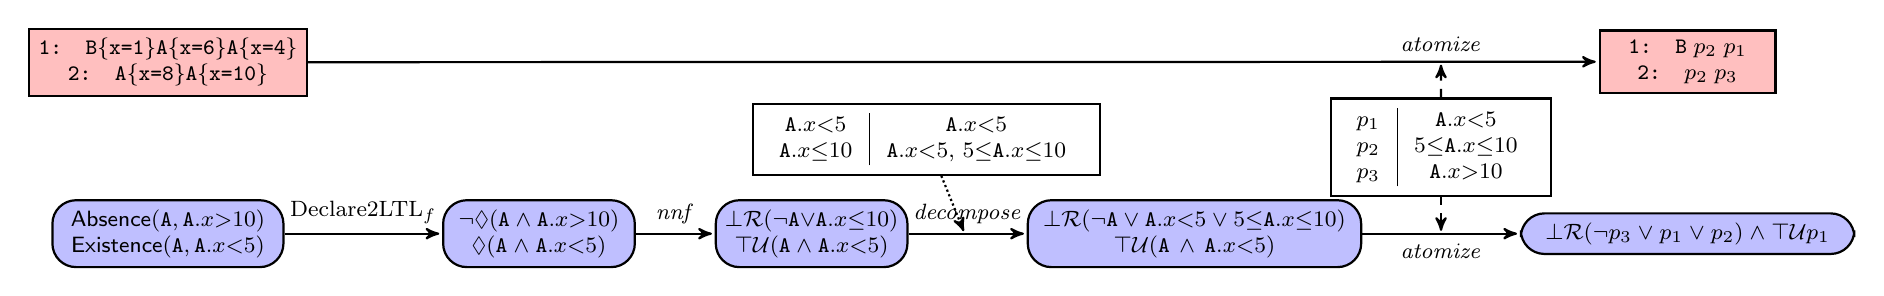
\begin{tikzpicture}[->,>=stealth',shorten >=1pt,thick,initial text=$ $,align=center,node distance=5mm,font=\footnotesize]
\thickmuskip=0mu
%% Input
\node (Clause)  [fill=blue!25,text width=2.7cm,rounded corners=.3cm,draw=black] 
				{$\mathsf{Absence}(\texttt{A},\;\texttt{A}.x>10)$\\
				 $\mathsf{Existence}(\texttt{A},\;\texttt{A}.x<5)$};
			 
%% Straightforward translation
\node (LTLf1) 
				[right=2cm of Clause,fill=blue!25,text width=2.2cm,rounded corners=.3cm,draw=black] 
				{$\neg\lozenge(\texttt{A}\wedge \texttt{A}.x>10)$\\
				 $\lozenge(\texttt{A}\wedge \texttt{A}.x<5)$};
\draw[->] (Clause) -- (LTLf1) node[midway,above] {Declare2LTL$_f$};
				
%% Conversion to NNF				
\node (LTLf2) 	[right=1cm of LTLf1,fill=blue!25,text width=2.2cm,rounded corners=.3cm,draw=black] 
				{$\bot\;\mathcal{R}\;(\neg\texttt{A}\vee  \texttt{A}.x\leq 10)$\\
				 $\top\;\mathcal{U}\;(\texttt{A}\wedge \texttt{A}.x<5)$};
\draw[->] (LTLf1) --  (LTLf2) node[midway,above] {\textit{nnf}};

%% Data predicates decomposition
\node (LTLf3) 	[right=1.5cm of LTLf2,fill=blue!25,text width=4cm,rounded corners=.3cm,draw=black] 
				{$\bot\;\mathcal{R}\;(\neg\texttt{A}\vee  \texttt{A}.x<5\vee 5\leq \texttt{A}.x\leq 10)$\\
				 $\top\;\mathcal{U}\;(\texttt{A}\wedge \texttt{A}.x<5)$};
\draw[->] (LTLf2) --  (LTLf3) node[midway,above] {\textit{decompose}};

\node (tab1) [ shape=rectangle,draw] at ($(LTLf2)!0.3!(LTLf3)+(0,1.2)$) {
	\begin{tabular}{c|c}
	$\texttt{A}.x<5$      & $\texttt{A}.x<5$\\
	$\texttt{A}.x\leq 10$ & $\texttt{A}.x<5$, $5\leq \texttt{A}.x\leq 10$\\
	\end{tabular}
};
\draw[->,densely dotted] (tab1) -- ($(LTLf2)!0.4!(LTLf3)$);

\node (LTLf4) 	[right=2cm of LTLf3,fill=blue!25,text width=4cm,rounded corners=.3cm,draw=black] 
				{$\bot\;\mathcal{R}\;(\neg p_3\vee  p_1\vee p_2)\wedge \top\;\mathcal{U}\; p_1$};


\node (CTraces) [fill=red!25,text width=2cm,draw=black,above=1.5cm of LTLf4] 
                {\texttt{1:\quad B\;$p_2$\;$p_1$}\\
                 \texttt{2:}\quad $p_2$\;$p_3$};

%\node[state,initial] (SA) at ($(LTLf4)-(1.3,3.5)$) {$s_1$};
%\path (SA) edge[loop] node[midway,above] (W1) {$\Sigma\backslash\{p_1,p_3\}$} (SA);
%\node[state,accepting,right =2cm of SA] (ST) {$s_2$};
%\path (ST) edge[loop] node[midway,above] (W2) {$\Sigma\backslash\{p_3\}$} (ST);
%\draw[->] (SA) -- (ST) node[midway,above] {$\{p_1\}$};
%\node[state] (bot) at ($(SA)!0.5!(ST)-(0,2.5)$) {$\bot$};
%\draw[->] (SA) -- (bot) node[midway,below,sloped] {$\{p_3\} $} ;
%\draw[->] (ST) -- (bot) node[midway,below,sloped] {$\{p_3 \}$} ;
%\draw (bot) to [in=225,out=315,looseness=8] node[midway,above] (W3) {$\Sigma$} (bot);
%\node[draw=black,fit=(SA) (ST) (W1) (W2) (bot) (W3)] (NFA) {};

\node (Traces) [fill=red!25,text width=3.3cm,draw=black,above=1.3cm of Clause] 
               {\texttt{1:\quad B\{x=1\}A\{x=6\}A\{x=4\}}\\
               	\texttt{2:\quad A\{x=8\}A\{x=10\}}};

\draw[->] (LTLf3) -- (LTLf4) node[midway,below]  {\textit{atomize}};




\draw[->] (Traces) -- (CTraces);
\node (tab2) [shape=rectangle,draw] at ($(LTLf4)!0.5!(LTLf3)+(0,1.1)$) {
	\begin{tabular}{c|c}
	$p_1$ &  $\texttt{A}.x<5$\\
	$p_2$ & $5\leq \texttt{A}.x\leq 10$\\
	$p_3$ &  $\texttt{A}.x>10$\\
	\end{tabular}
};

\draw[->,dashed] (tab2) -- ($(Traces)!(tab2.north)!(CTraces)$) node [above] {\textit{atomize}};
\draw[->,dashed] (tab2) -- ($(LTLf3)!0.5!(LTLf4)$);

%
%\draw[->] (LTLf4) -- (NFA) node[midway,left] {LTL$_f$2DFA};
  \end{tikzpicture}
\end{document}